% !TEX root = handbook-physics.tex
%!TEX TS-program = pdflatex
%!TEX encoding = UTF-8 Unicode

\chapter{Real Gases And Vapours}
\label{ch-12}


\section{Forces of Intermolecular Interaction}
\label{sec-12.1}

\subsection{}\label{12.1.1} The properties of gases that are not highly rarified differ from those of ideal gases, which comply with the Mendeleev- Clapeyron equation \ssect{8.4.4}. Experiments indicate that the specific heat capacities \ssect{9.5.2}, coefficients of viscosity \ssect{10.8.4} and other quantities have different values for real gases than for ideal gases.

\subsection{}\label{12.1.2} A \redem{real gas} is one in which forces of molecular interaction exist between the molecules.

A \redem{vapour} is a real gas in states close to that in which it con­denses.

\subsection{}\label{12.1.3} The forces of intermolecular interaction decrease rapidly with an increase in the distances between the molecules (\redem{short-range forces}). At intermolecu­lar distances exceeding \SI{d-9}{\meter},
these forces can be neglected. Forces of interaction between molecules can be subdivided into \redem{forces of attraction} and \redem{forces of repulsion}. Both types act simultaneously. Otherwise it would be impossible to deter­ mine the volume of liquids or solids: their constituent par­ticles would either fly apart in all directions or would stick together, forming the minimum possible volume.

\subsection{}\label{12.1.4} The forces of mutual attraction and repulsion depend differently on the distance r between the molecules. At dis­tances commensurable with the linear dimensions of atoms and small inorganic molecules
(\SI{d-10}{\meter}),repulsive forces $\vb{F}_{1}$ pre­dominate; at distances $r$ of the order of \SI{d-9}{\meter} forces of mutual attraction $\vb{F}_{1}$ prevail. If $\vb{r}$ is the radius vector to the point where molecule $A$ is located from a point where molecule $B$ is located and acts on molecule $A$ with the forces $\vb{F}_{1}$ and $\vb{F}_{2}$, then
\begin{equation*}%
\vb{F}_{1} = F_{1r} \frac{\vb{r}}{r} \qand \vb{F}_{2} = F_{2r} \frac{\vb{r}}{r} 
\end{equation*}
Projections $F_{1r}$ and $F_{2r}$ of forces $\vb{F}_{1}$ and $\vb{F}_{3}$ on the direction of $\vb{r}$ depend upon $r$ in the following way
\begin{equation*}%
F_{1r} = \frac{b}{r^{3}} \qand  F_{2r} = -\frac{a}{r^{7}} 
\end{equation*}
where $a$ and $b$ are factors that depend on the structure of the molecules and the type of intermolecular interaction. The curves in \figr{fig-12-01} show the dependence of $F_{1r}$ and $F_{2r}$ on $r$. Forces of repulsion are conventionally accepted as positive and at­ tractive forces as negative (\figr{fig-12-01}).

\begin{figure}[!ht]
\centering
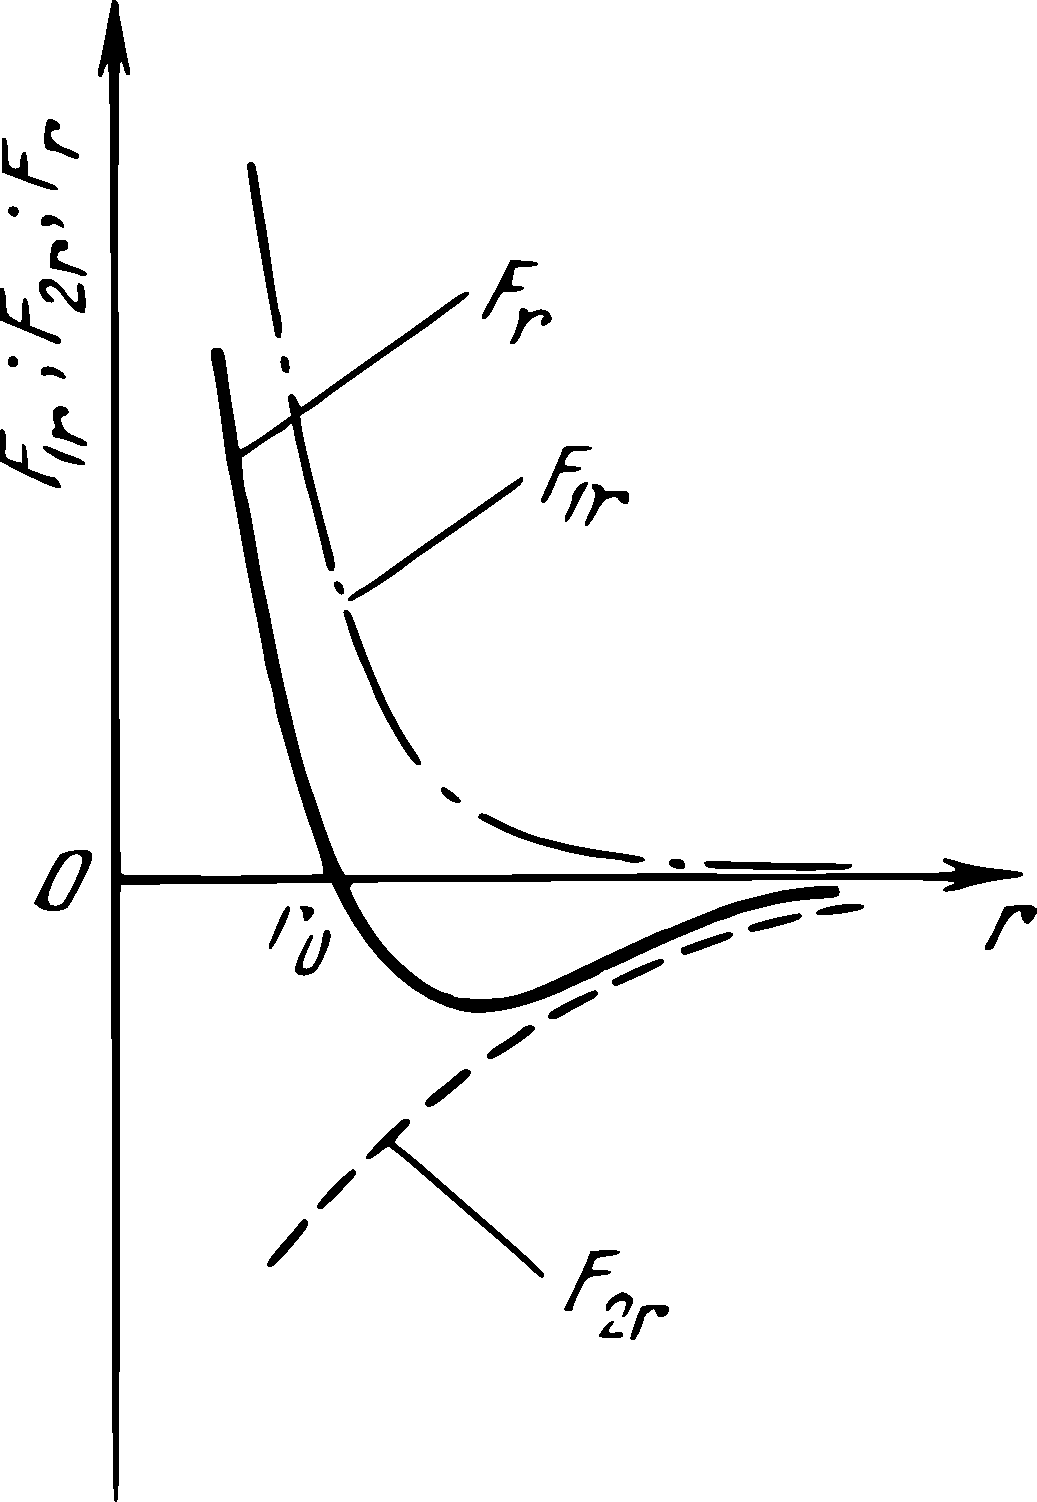
\includegraphics[width=0.4\textwidth]{figs/ch-12/fig-12-01.pdf}
\caption{Forces of attraction and repulsion for two molecules.}
\label{fig-12-01}
\end{figure}

The resultant force is 
\begin{equation*}%
\vb{F} = \vb{F}_{1} + \vb{F}_{2} = F_{r} \frac{\vb{r}}{r} 
\end{equation*}
and $F_{r} = F_{1r} + F_{2r}$. The dependence of $F_{r}$ on $r$ is also shown in \figr{fig-12-01}.

\subsection{}\label{12.1.5} At $r = r_{0}$, forces $\vb{F}_{1}$ and $\vb{F}_{2}$ counterbalance each other and $\vb{F} = 0$. At $r > r_{0}$ force $\vb{F}_{2} > \vb{F}_{1}$ at $r < r_{0}$ force $\vb{F}_{2} < \vb{F}_{1}$. Thus $r_{0}$ is the equilibrium distance between the molecules and where they would be with respect to each other if there were no thermal motion.

\subsection{}\label{12.1.6} The element of work $\delta W$ done by the resultant force $\vb{F}$, when the distance between the molecules is increased by the amount $\dd \vb{r}$, is equal to the decrease in the mutual potential energy $E_{p}$ of the two molecules \ssect{3.3.1}:
\begin{equation*}%
\delta W = (\vb{F},\, \dd \vb{r}) = F_{r} \, \dd r = - \dd E_{p}
\end{equation*}
Integrating with respect to $r$ from $r$ to $\infty$:
\begin{equation*}%
\int_{E_{p}}^{E_{p}\infty} \dd E_{p} = - \int_{r}^{\infty} F_{r} \, \dd r \qand  E_{p} - E_{p \infty} = \int_{r}^{\infty} F_{r} \, \dd r
\end{equation*}
At $r = \infty$ the molecules do not interact and $E_{p} - E_{p \infty} = 0$. Hence,
\begin{equation*}%
E_{p} = \int_{r}^{\infty} F_{r} \, \dd r
\end{equation*}
This integral can be calculated graphically from the known de­pendence of $F_{r}$ on $r$ (\figr{fig-12-01}). It is proportional to the area bounded by the curve $F_{r} = F_{r}\,(r)$, the $r$ axis and the value of $r$ (where $r = \textrm{const}$) for which $E_{p}$ is being calculated. At $r > r_{0}$, the energy $E_{p} < 0$ because $F_{r} < 0$; at $r = r_{0}$, the energy $E_{p}$ reaches its minimum value: $E_{p} = E_{\textrm{min}}$. This follows from the equation
\begin{equation*}%
\left( \frac{\dd E_{p}}{\dd r}\right)_{r = r_{0}} = - F_{r}(r_{0}) = 0.
\end{equation*}
A system consisting of the interacting molecules, in a state of stable equilibrium ($r= r_{0}$),possesses minimum potential energy. At $r < r_{0}$, the energy $E_{p}$ begins to increase, becomes positive and then rises drastically due to the rapid increase in the repulsive forces as r drops (\figr{fig-12-02}).

\begin{figure}[!ht]
\centering
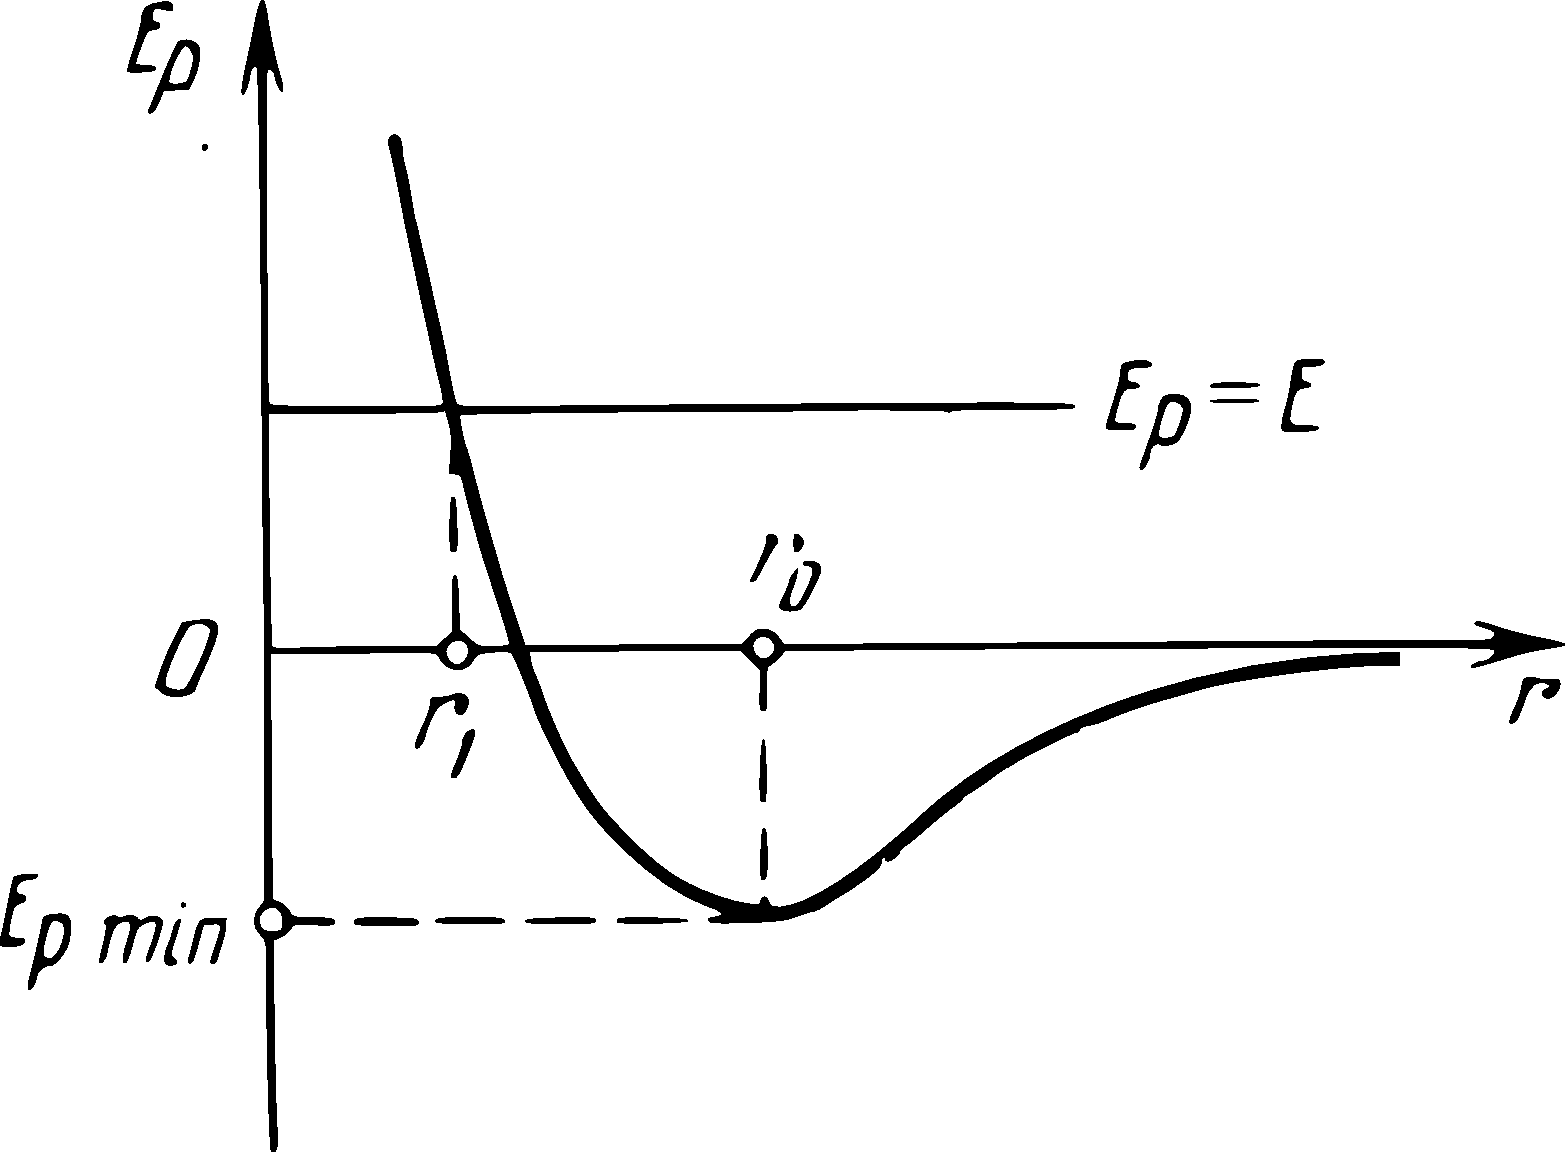
\includegraphics[width=0.6\textwidth]{figs/ch-12/fig-12-02.pdf}
\caption{Energy $E_{p}$ and distance.}
\label{fig-12-02}
\end{figure}

\subsection{}\label{12.1.7} The value $E = E_{p \textrm{min}}$, the minimum potential energy of interaction of molecules, is the criterion for various states of aggregation of matter.

If $\abs{\,E\,}_{p \textrm{min}} \ll kT$, the substance is in a gaseous state. When $\abs{\,E\,}_{p \textrm{min}} \gg kT$, it is in the solid state. The condition $\abs{\,E\,}_{p \textrm{min}} \approx kT$ corresponds to the liquid state. Here $kT$ is twice the average energy per degree of freedom of thermal motion of the molecules \ssect{10.6.4}.

\subsection{}\label{12.1.8} \redem{Van der Waals} forces are weak\sidenote{Weak in the sense of their small magnitude compared to the forces of attraction that provide for the formation of stable molecules \ssect{12.1.9}.} forces of attraction that act between molecules at distances of the order of \SI{d-9}{\meter} \ssect{12.1.4}. They are the reason for the correction of the internal pressure in the Van der Waals equation of state for a real gas \ssect{12.2.4}. Distinction is made between three types of Van der Waals forces of attraction.
\begin{enumerate}[label=(\alph*),noitemsep,nolistsep]
\item Orientational forces of attraction $\vb{F}_{or}$ are due to the fact that asymmetric polar molecules \ssect{18.1.4} have constant dipole moments $p_{e}$ \ssect{18.1.4}. The result of interaction of these dipole moments is the attraction force $\vb{F}_{or}$. This force is opposed by the thermal motion of the molecules. Calculations indicate that
\begin{equation*}%
\vb{F}_{or} \propto - \frac{p_{e}^{4}}{kT} \frac{1}{r^{7}}
\end{equation*}
where $r$ is the distance between the molecules, $k$ is Boltzmann's constant \ssect{8.4.5}, and $T$ is the absolute temperature.
\item \redem{Induction forces} of attraction are exerted when a neutral molecule of a real gas is in an electric field set up by another molecule, both molecules having high polarizability \ssect{18.1.3}. If the molecules are sufficiently close together, the action of the electric field of the second molecule develops an induced dipole moment $\vb{p}_{e} = \epsilon_{0} \beta \vb{E}$ \ssect{18.1.4} in the first molecule, where $\beta$ is the polarizability of the molecule \ssect{18.1.3}, and $\vb{E}$ is the strength of the electric field set up by the second molecule. To constant factors
\begin{equation*}%
\vb{F}_{in} \propto - \beta p_{e}^{2} \frac{1}{r^{7}}
\end{equation*}
\item The vibration of electrons in one molecule (or atom) can excite vibration in another molecule (or atom). The vibrations of the electrons in the two molecules are in phase with each other, leading to attraction between the molecules (or atoms). The resulting resonance forces of attraction are called \redem{disper­sion forces}. They play the main role in the interaction of non­ polar molecules \ssect{18.1.3}. The force of dispersion attraction is
\begin{equation*}%
\vb{F}_{d} \propto - \beta \frac{e^{4}h\nu_{0}}{k^{2}} \frac{1}{r^{7}}
\end{equation*}
where $e$ is the charge of the electron, $h$ is Planck's constant,
$\nu_{0}= (1/2\pi) \sqrt{k/m}$ is the frequency of vibration of the atoms \ssect{28.1.2}, $k$ is the coefficient of the quasi-elastic force \ssect{40.3.7}, and $m$ is the mass of the atom.
\end{enumerate}
Dispersion forces owe their name to the analogy between the origin of these forces and dispersion phenomena occurring when electromagnetic waves propagate through matter \ssect{34.4.1}.


\subsection{}\label{12.1.9} The attraction force $\vb{F}_{r}$ between two molecules, shown in \figr{fig-12-01}, is the resultant of all the kinds of attraction enumerated in \ssect{12.1.8}. The potential energy of Van der Waals attraction amounts to (0.4 to 4) \times \SI{d3}{\joule\per\mole}.

In addition to the electromagnetic interaction, a special kind of quantum interaction exists between molecules at distances $r < \SI{d-10}{\meter}	$. This interaction leads either to the development of repulsive forces between the molecules \ssect{12.1.4}, or to strong attraction of adjacent atoms (or groups of atoms) and the for­mation between them of ionic and covalent chemical bonds (\ssect{39.4.4} and \ssect{39.4.5}). The result of such bonds is the formation of stable molecules. The potential energy of chemical bonds exceeds the energy of Van der Waals attraction and ranges from (0.4 to 4) \times \SI{d4}{\joule\per\mole}.

\subsection{}\label{12.1.10} Being internal forces \ssect{2.2.4}, the forces of interaction in a system of two molecules cannot change the total energy $E$ of the system, which is the sum of the kinetic energy $E_{k}$ of the molecules and their mutual potential energy $E_{p}$. Hence
\begin{equation*}%
\dd E = \dd E_{k} + \dd E_{p} = 0 \qor \dd E_{k}  = - \dd E_{p} = F_{r} \dd r
\end{equation*}
Use is made here of the equation in \ssect{12.1.6}. When the molecules are brought closer together $(\dd r < 0)$, to the distance $r_{0}$ (\figr{fig-12-01}), the potential energy $E_{p}$ decreases and the kinetic energy $E_{k}$ accordingly increases. This occurs at the expense of the positive work done by the resultant force of mu­tual attraction between the molecules \ssect{12.1.4} ($F_{r} < 0$ when $r > r_{0}$). As the molecules are brought still closer, they do work in overcoming the resultant force of mutual repulsion ($F_{r} > 0$ when $r < r_{0}$). This reduces the kinetic energy of the molecules. At the instant they are closest together ($r = r_{1}$ in \figr{fig-12-02}) all of the kinetic energy of the molecules has been completely expended in doing work to overcome the repulsive forces:
$E_{k} = 0$ and the total energy $E$ is equal to the potential energy $E_{p}$, i.e. $E = E_{p}$ (\figr{fig-12-02}).

If all the state variables of real gases are maintained constant with the exception of the temperature, the distance $r_{1}$ decreases when the gas is heated. This decrease is very small, however, even at high temperatures. This is due to the extremely steep increase in the repulsive forces $F_{1}$ as $r$ is decreased (\figr{fig-12-01}). Thus the distance $r_{1}$ is the effective diameter $d$ of the molecule \ssect{8.4.1}. The finite dimensions of molecules of real gases are explained by the action of repulsive forces between the mol­ecules.


\section{Van der Waals Equation of State}
\label{sec-12.2}

\subsection{}\label{12.2.1} A \redem{Van der Waals gas} is a model of a real gas in which the molecules are dealt with as perfectly rigid spheres of diam­eter $d$ \ssect{12.1.10}, with forces of mutual attraction acting between them. The finite size of the spheres signifies that the repulsive forces between the molecules of a real gas are also taken into account.

\subsection{}\label{12.2.2} The molecules of a real gas, each having a volume of $\tilde{v} = \pi d^{3}/6$, do not move around as freely in a vessel as the ``point'' molecules of an ideal gas. Therefore, in the Mendeleev-Clapeyron equation \ssect{8.4.4} $pV = RT$, the total volume $V$ of a vessel holding one mole of the gas should be replaced by the ``free'' volume
\begin{equation*}%
V'_{\mu} = V_{\mu} - b
\end{equation*}
where $b$ is Van der Waals's correction for the intrinsic volume of the molecules. Correction $b$ is equal to four times the volume of all the molecules contained in one mole of the gas:
\begin{equation*}%
b = 4N_{A} \tilde{v}
\end{equation*}
where $N_{A}$ is Avogadro's number (Appendix~II), and $\tilde{v}$ is the volume of a single molecule.

\subsection{}\label{12.2.3} The forces of mutual attraction between the molecules are taken into account for a Van der Waals gas by introducing a correction for the pressure in the Mendeleev-Clapeyron equa­tion \ssect{8.4.4}. Owing to the short-range nature of the attraction forces \ssect{12.1.3}, each molecule interacts only with particles that are located at distances $r \leqslant R_{m}$, where $R_{m}$ is the \redem{range of molecular action}, with a magnitude of the order of \SI{d-9}{\meter}. A sphere of radius $R_{m}$ is called the \redem{sphere of molecular action}.

The forces of attraction of a molecule within the bulk of the gas to other molecules are mutually counterbalanced and have no effect on the motion of the given molecule. If the molecule is within a layer of gas that borders on a wall of the vessel, it is subject to an uncompensated force of attraction directed inward, into the bulk of the gas. Consequently, in its collision with a wall, such a molecule imparts less momentum to the wall \ssect{10.2.1}, and the pressure $p$ exerted by a real gas on the walls is reduced in comparison to the pressure $p$ of an ideal gas having the same density at the same temperature,
\begin{align*}%
p & = p_{id} - p^{*} \qor\\
p_{id} & = p + p^{*}
\end{align*}
where $p*$ is the Van der Waals correction due to the forces of mutual attraction and is called the \redem{internal pressure}. The inter­nal pressure $p^{*}$ is inversely proportional to the square of the volume of the vessel occupied by one mole of the gas:
\begin{equation*}%
p^{*} = \frac{a}{V_{\mu}^{2}}
\end{equation*}
where $a$ is the Van der Waals coefficient and depends upon the chemical nature of the gas.

\subsection{}\label{12.2.4} The Van der Waals equation describes the state of a real gas and differs from the Mendeleev-Clapeyron equation \ssect{8.4.4} in that the corrections $b$ and $p*$ have been introduced (\ssect{12.2.2} and \ssect{12.2.3}). For a single mole of gas it is of the form
\begin{equation*}%
\left( p + \frac{a}{V_{\mu}^{2}} \right) \, (V_{\mu} - b) = RT
\end{equation*}

\subsection{}\label{12.2.5} The Van der Waals equation for an arbitrary mass of real gas, having the molar mass $p$ \ssect{8.4.3}, is
\begin{equation*}%
\left( p + \frac{M^{2}}{\mu^{2}} \, \frac{a}{V^{2}} \right) \, \left(V - \frac{M}{\mu} b \right) = \frac{M}{\mu} \, RT
\end{equation*}
This equation is valid for gases that are not too highly compressed. In highly rarefied gases $V_{\mu} \gg B$, $p^{*} \ll p$ and the Van der Waals equation does not differ from the Mendeleev-Clapeyron equation.

\section{Isothermals of Real Gases. Phase Transitions}
\label{sec-12.3}

\subsection{}\label{12.3.1} The curve representing the dependence of the molar volume of a gas on the pressure at constant temperature is called the \redem{isothermal}, or \redem{isotherm}, of a real gas. Isothermals of carbon dioxide gas are shown in \figr{fig-12-03}. At temperatures $T$ below $T_{C} = \SI{340}{\kelvin}$, all the isothermals have horizontal steps along which, in addition to the constant temperature, the pressure is also constant while the molar volume varies. The difference $V_{D} - V_{B}$ of the molar volumes over the horizontal steps de­creases as the temperature is raised \figr{fig-12-03}. At $T = T_{c}$ this difference vanishes. The temperature $T = T_{c}$ , corresponding to the condition $V_{D} - V_{B} = 0$, is called the \redem{critical temperature}. The isothermal of a real gas at $T = T_{c}$ is called the critical isothermal. On this isothermal points $D$ and $B$ merge into point $C$, which is called the \redem{critical point}. The state variables \ssect{8.3.2} of the gas at the critical point are the critical variables $V_{\mu c}$, $p_{c}$ and $T_{c}$.

\begin{figure}[!ht]
\centering
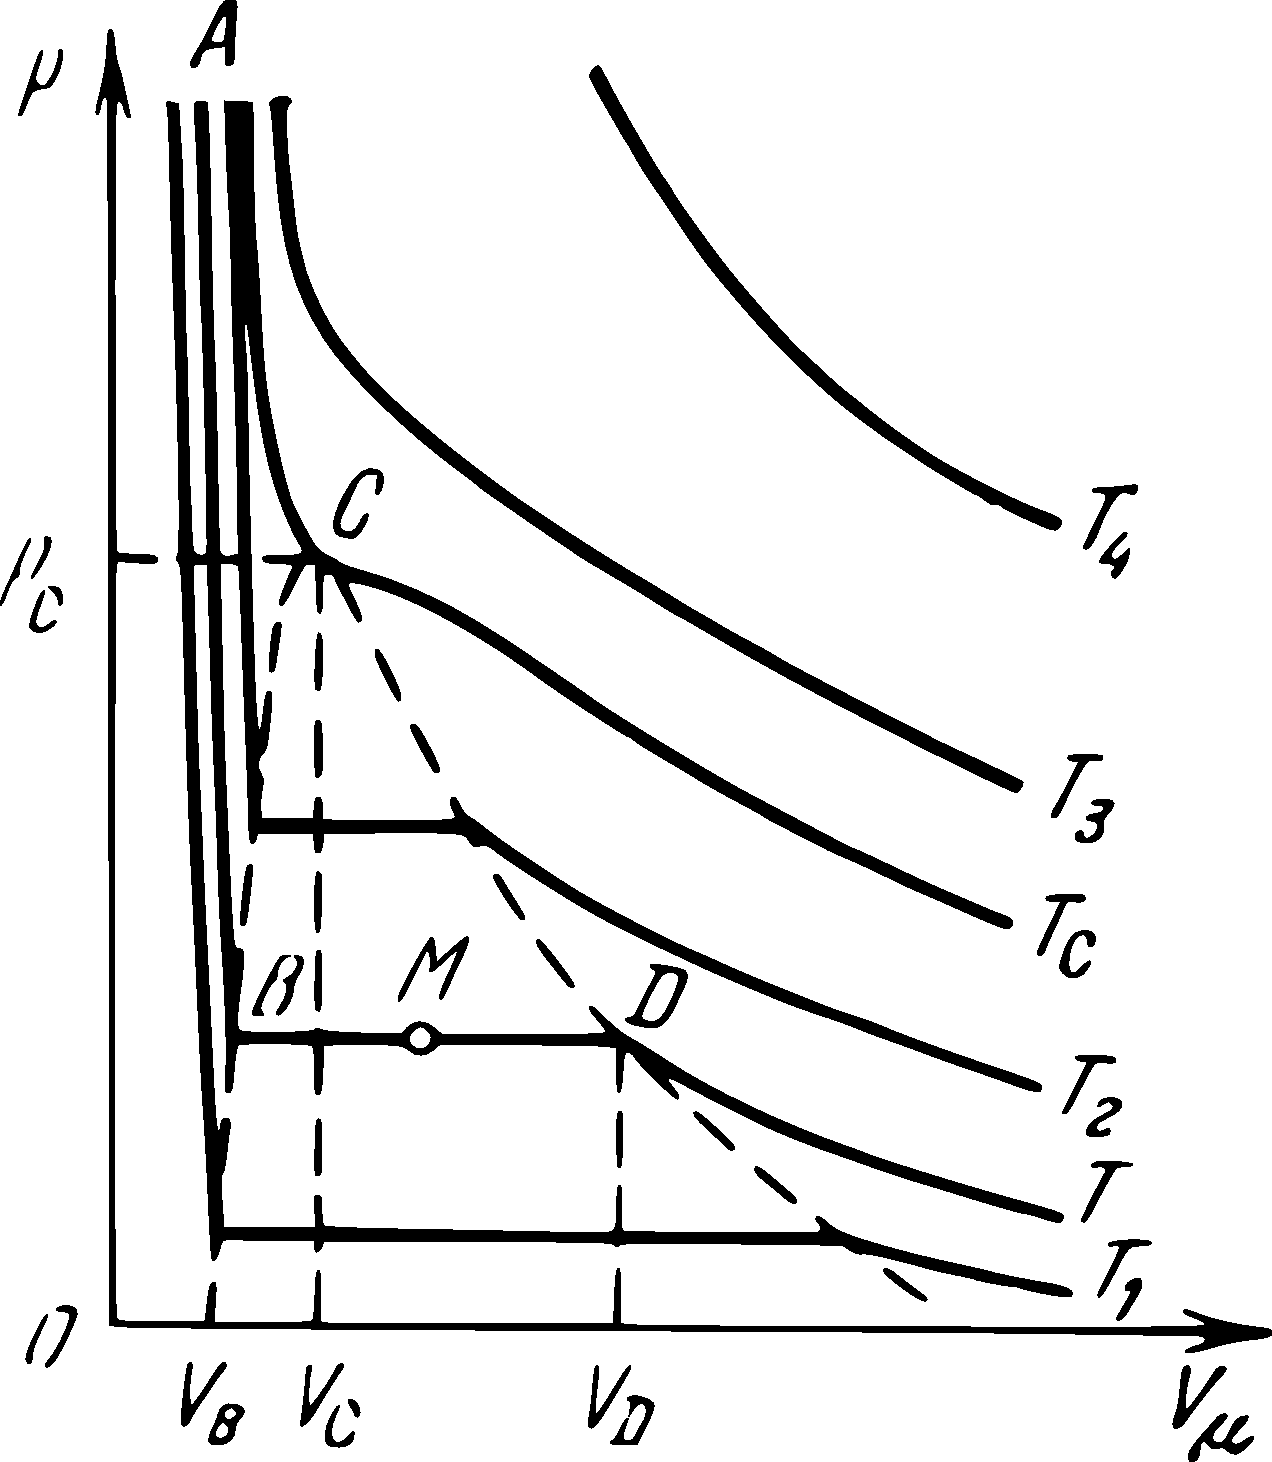
\includegraphics[width=0.5\textwidth]{figs/ch-12/fig-12-03.pdf}
\caption{Isothermals of carbon dioxide gas.}
\label{fig-12-03}
\end{figure}

Critical point $C$ is an inflection point on the critical isothermal.
Consequently, the tangent to the isothermal at this point is parallel to the $OV_{\mu}$ axis.

\subsection{}\label{12.3.2} Any subcritical isothermal $(T < T_{c})$ is a curve representing the continuous transition of the substance from the gaseous to the liquid state. It consists of three portions: $TD$, $DB$ and $BA$, each of which represents different states of the substance. Over the portion $TD$ the substance is in the gaseous state, portion $DB$ corresponds to the transition of the substance from the gaseous to the liquid state. Over the portion $BA$ of the isothermal, the substance is a liquid. This portion is almost vertical owing to the low compressibility of liquids. Points $D$ and $B$ of the horizontal portion of the isothermal correspond to the beginning and end of condensation in isothermal compression of a real gas. On the contrary, in isothermal expansion of the liquid, points $B$ and $D$ are the beginning and end of the boiling process. Point $B$ corresponds to the state of a \redem{boiling liq­uid}, point $D$ to \redem{dry saturated vapour}. The mixture of the boiling liquid and dry saturated vapour that exists at any point $M$ of portion $BD$ is called wet vapour (\figr{fig-12-03}).

\subsection{}\label{12.3.3} In thermodynamics a \redem{phase} is a totality of all the parts of a system, having the same chemical composition and being in the same state. Wet vapour, for instance, is a two-phase sys­tem consisting of boiling liquid and dry saturated vapour.


\begin{marginfigure}[!ht]
\centering
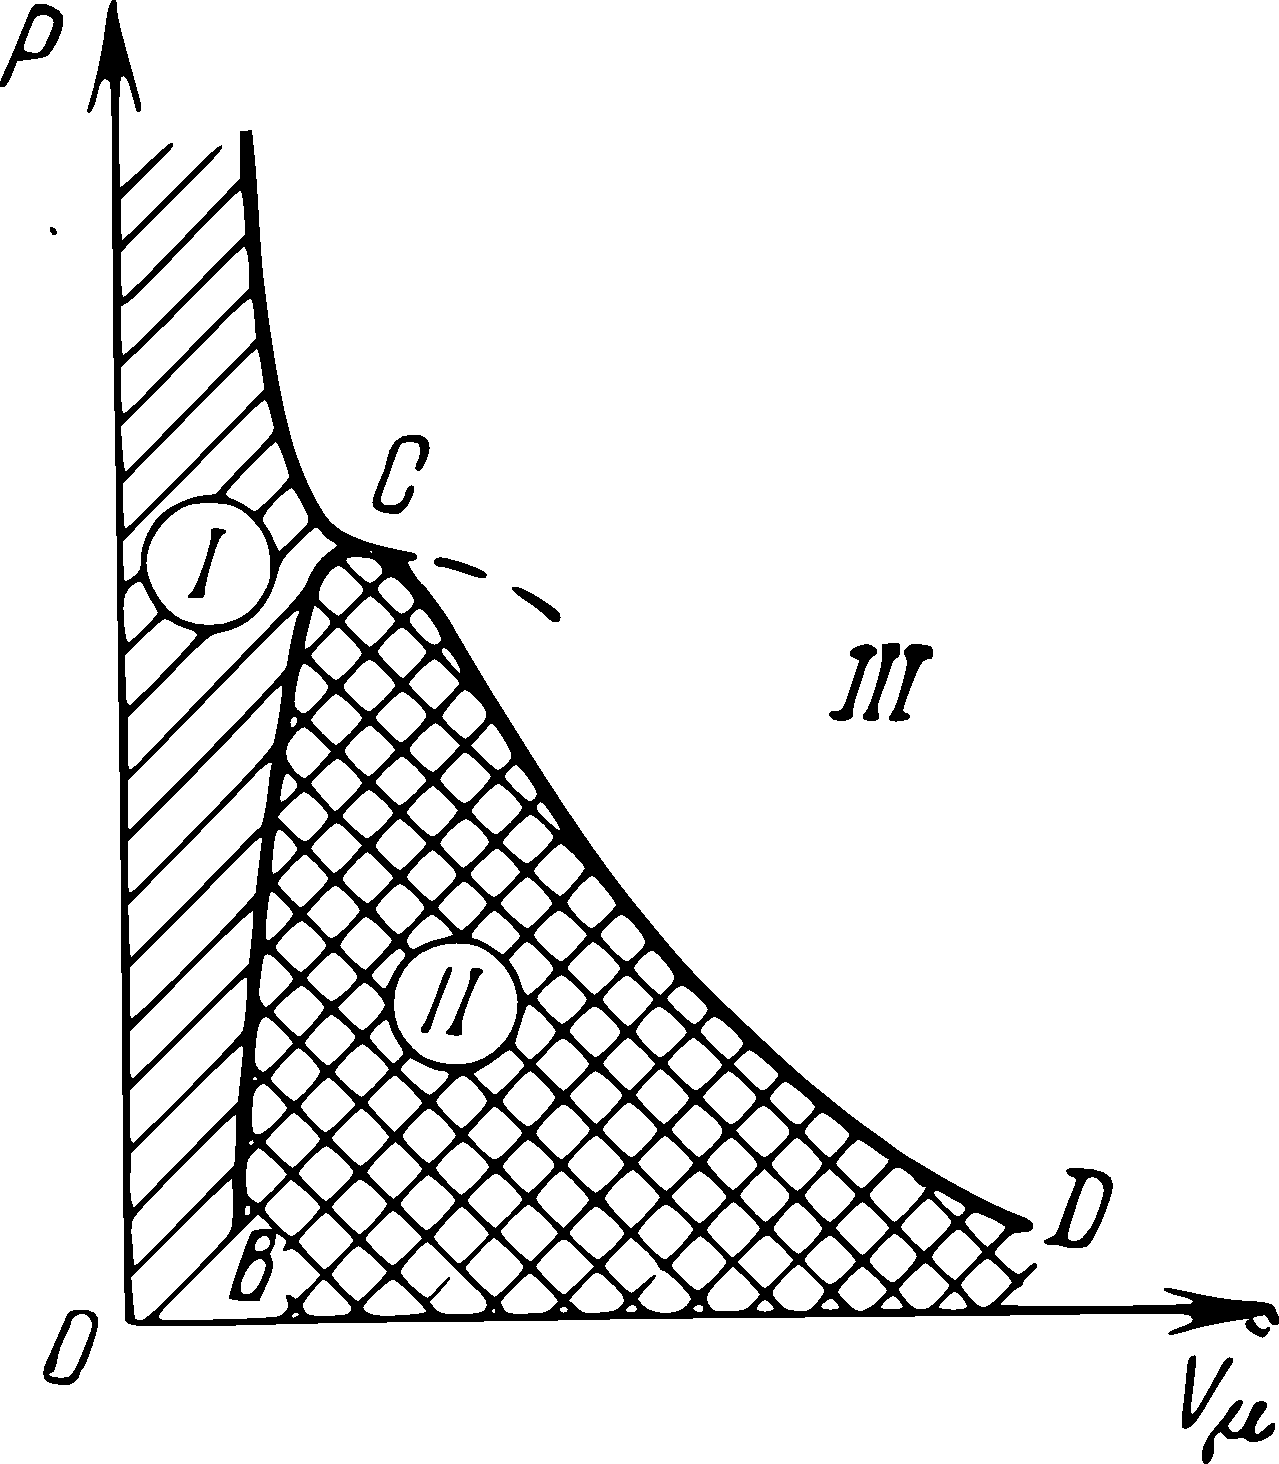
\includegraphics[width=0.8\textwidth]{figs/ch-12/fig-12-04.pdf}
\caption{Phases.\label{fig-12-04}}
\end{marginfigure}

Shown in \figr{fig-12-04} are two boundary curves $BC$ and $DC$ which connect points $B$ and $D$ (\figr{fig-12-03}) at various temperatures. Curves $BC$ and $DC$ converge at critical point $C$. Boiling curve $BC$ separates the single-phase liquid region $I$ from the two- phase wet vapour region $II$. The curve $BC$ is one representing the beginning of the \redem{first-kind phase} transition of the substance from the liquid to the gaseous state. The boundary curve $DC$ separates the two-phase region $II$ from the single-phase region $III$ in which the substance is in the gaseous state.

\subsection{}\label{12.3.4} The two-phase region $II$ cannot exist at pressures above the critical one $p_{c}$ \ssect{12.3.1} at which the substance can be in either of two states, gaseous or liquid. No pressure can convert gas at a temperature above the critical $T_{c}$ into the liquid state by isothermal compression. The critical temperatures of many gases are very low: $T_{c} \approx \SI{5}{\kelvin}$ for helium and \SI{33}{\kelvin} for hydro­gen. This makes the liquefaction of such gases quite difficult. 

\subsection{}\label{12.3.5} Besides the difference in the molar volumes of boiling liquid and dry saturated vapour, the specific heat of vaporizalion \ssect{13.6.4} also vanishes when a substance is in the critical state, as does the surface tension \ssect{13.4.4}. The difference between the liquid and gaseous states of a substance completely disappears when it is in the critical state.

\subsection{}\label{12.3.6} The Van der Waals equation \ssect{12.2.4} is a cubic equation with respect to the molar volume $V$, having factors that depend upon the pressure, temperature and the chemical nature
of the gas. This equation has either one or three real roots, in accordance with the numerical values of $p$ and $T$. Shown in \figr{fig-12-05} are the isothermals of a real gas that complies with the Van der Waals equation. The isothermals correspond to the different temperatures $T_{1} < T_{2} < T_{3} < T_{c} < T_{5} < T_{6}$. All the subcritical isothermals have a hatched portion where each pressure corresponds to three different states, which are represented by the three points, $B$ , $E$ and $G$, of the isothermal.

\begin{marginfigure}%[!ht]
\centering
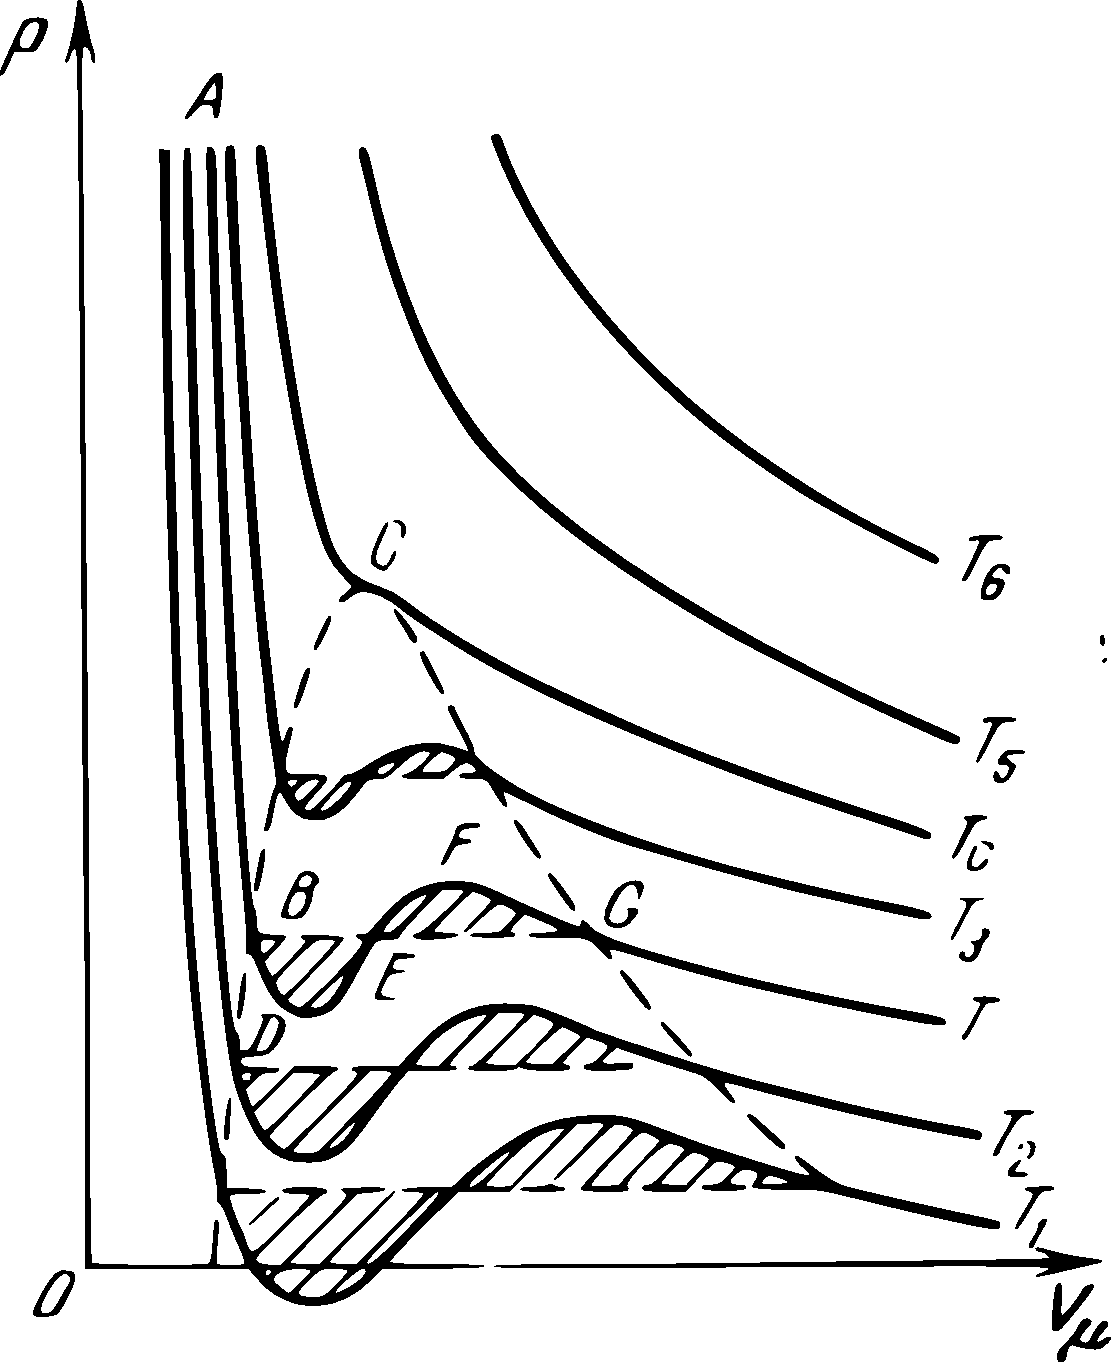
\includegraphics[width=0.5\textwidth]{figs/ch-12/fig-12-05.pdf}
\sidecaption{Isothermals of a real gas that compling with the Van der Waals equation.
\label{fig-12-05}}
\end{marginfigure}

The wave-shaped portion $BDEFG$ of the isothermal in \figr{fig-12-05} more accurately represents the transition of the substance from (lie gaseous to the liquid state than the horizontal portions of experimentally plotted isothermals (dash straight lines $BG$). The portion $BD$ of the isothermal corresponds to a \redem{superheated liquid}, which can be obtained if the beginning of boiling is delayed at point $B$. The portion $GF$ of the isothermal represents the state of \redem{supersaturated vapour}, occurring upon slow isothermal compression in the absence of condensation centres. If such centres (dust specks or ions) are introduced into the supersatu­rated vapour, extremely rapid condensation of the vapour takes place. Over the portion $DEF$, the molar volume increases (decreases) as the pressure is increased (decreased). Such states of matter are impossible. The horizontal steps $BG$ cut the portions $BDEFG$ of the isothermals in such manner that the hatched areas $BDEB$ and $EFGE$ in \figr{fig-12-05} are equal to each other (\redem{Max­well's equal area rule}).

\subsection{}\label{12.3.7} The values of the critical variables $p_{c}$, $V_{\mu \, c}$ and $T_{c}$ \ssect{12.3.1} can be expressed in terms of the coefficients $a$ and $b$ in the Van der Waals equation \ssect{12.2.4} and the universal gas constant $R$ \ssect{8.4.4}:
\begin{equation*}%
p_{c} = \frac{1}{27} \, \frac{a}{b^{2}}, \quad V_{\mu \, c} = 3b	, \qand T_{c} = \frac{8}{27} \, \frac{a}{bR}.
\end{equation*}

\section{Superfluidity Of Helium}
\label{sec-12.4}


\subsection{}\label{12.4.1} Helium is a kind of substance which, after going over from the gaseous to the liquid state at standard atmospheric pressure and a temperature of \SI{4.22}{\kelvin}, remains in the liquid state no matter how close to absolute zero \ssect{11.8.4} it is cooled. 

\subsection{}\label{12.4.2} At the temperature \SI{2.19}{\kelvin} a second-order phase transi­tion occurs: liquid helium I, existing at temperatures $T > \SI{2.19}{\kelvin}$, undergoes the transition to liquid helium II, which exists at $T < \SI{2.19}{\kelvin}$.

A \redem{second-order phase transition} is a transformation of matter that is not associated with the evolution or absorption of heat as in a first-order transition. In second-order phase transitions the heat capacity, coefficient of thermal expansion and certain other characteristics of substances vary with discontinuous jumps. Some examples of second-order phase transitions are the transition of iron at the Curie point \ssect{26.5.2} from a ferro­-magnetic substance into a paramagnetic one \ssect{26.3.5} and the transition of certain metals and alloys at extremely low tem­peratures to the superconductive state \ssect{41.6.1}.

\subsection{}\label{12.4.3} \redem{Superfluidity}, a phenomenon observed \redem{in liquid he­lium II}, is the practically complete absence of viscosity when such helium flows through narrow capillary tubes \ssect{13.5.5}. The coefficient of viscosity \ssect{10.8.4} of helium II is less than \SI{d-12}{\pascal\second}, while that of helium I close to the temperature \SI{4.22}{\kelvin} is of the order of \SI{d-6}{\pascal\second}.

\subsection{}\label{12.4.4} According to the \redem{two-fluid theory}, liquid helium II is a mixture of a superfluid component and a normal component. The superfluid component moves without friction and does not participate in the transfer of energy in the form of heat \ssect{9.2.1}. The normal component moves with friction and does participate in energy transfer.

\subsection{}\label{12.4.5} The theory of superfluidity is based on quantum mechan­ics \ssect{38.1.2}. In the first place, quantum mechanics was required to explain why helium is the only nonfreezing liquid at ultra-low temperatures and standard pressure. The zero-point vibra­tions \ssect{38.5.6} of the light-weight atoms of helium are sufficient­ly intensive and do not allow the weak forces of attraction between the helium atoms to form a crystalline structure at ordinary pressures.

The present-day theory of superfluidity is based on a study of the energy spectrum of helium at ultra-low temperatures. Under these conditions the continuous energy spectrum can be regarded as the totality of quasi-particles with the energies $h \nu_{i}$, where $h$ is Planck's constant and $\nu_{i}$ is the phonon frequency \ssect{41.7.5} corresponding to these quasi-particles. The quasiparticles cannot be identified with the real atoms of helium. They repre­sent the motion of the whole system of helium atoms, and the energy values of the quasi-particle describe the energy spectrum of the whole quantum system, i.e. the liquid helium as a whole. 

At low temperatures the excited state of the helium constitutes sound waves that are quasi-particles in the normal part of he­lium II. Associated with the quasi-particles are the store of internal energy and the presence of friction in the liquid he­lium. But states are possible in helium II t hat correspond to its superfluid part, in which quasi-particles are not advantageous from the energy point of view and do not arise. As a result of the strong interaction between the particles of the superfluid part of helium II a bound body is formed in which no thermal excitations are generated: the superfluid part of helium II has no store of internal energy and is not subject to viscosity. At absolute zero temperature, there should actually not be any normal part in helium II; all of the helium should be superfluid. As the helium is heated, the number of phonons increases as does the share of the normal part of helium II. But until the temperature reaches \SI{2.19}{\kelvin}, a superfluid part of helium II, with its characteristic properties, still remains. At the temper­ature \SI{2.19}{\kelvin}, helium II is converted into helium I and all the special properties of helium II disappear.
